\section{Solving Cluster Imbalancedness}
As we previously stated, our approach depends to a certain extent on the level of balancedness of barcode classes and the culprit of the occasional unsatisfying performance appears to be data imbalancedness. An ideal situation for our algorithm would be the one where each barcode appears in equal number of reads, because most of the commonly used clustering algorithms are designed to finding balanced clusters. This is not surprising - if we take, for example, the graph clustering point of view which we discussed in Section \ref{sec:spectral_clustering}, the best cuts are sometimes meaningless from the point of clustering, because they consist of isolating one vertex as a singleton cluster \cite{von2007tutorial}. The assumption of balanced classes is, of course, very limiting and the experimenter has most of the times no control over the distribution of barcodes.

Qian et al. \cite{qian2013spectral} were first to have addressed this problem in spectral clustering. In their work they proved that spectral clustering algorithms that minimize \textbf{NCut}\footnote{or also \textbf{RCut}, which we do not mention in this thesis, but can be found in \cite{von2007tutorial}} yield clusterings of different qualities on imbalanced datasets for different choices of the input graph parameters ($k, \sigma, \epsilon$). They defined a new notion of a cut a graph $G = (V, E, W)$ that goes by the name \textit{Partition Constrained Min-Cut} - \textbf{PCut}. For simplicity, we introduce it for  only two clusters as Quan et al. did, but it can be trivially generalized for any number of clusters \cite{qian2013spectral}:

\begin{equation}
    \textbf{PCut} = \arg \min_{A \in \mathcal{P}(V)} \{
        \textbf{Cut}(A, \overline{A} ~|~ min(|A|, |\overline{A}|) \geq \delta |V| )
    \},
    \label{eq:pcut}
\end{equation}
where $\mathcal{P}(V) = \{S ~|~ S \subseteq V\}$.

Hence, objective of \textbf{Pcut} in Eq. \ref{eq:pcut} is to find a \textbf{Cut} of optimal value among the cuts that do not yield clusters too small in size. The size of the smallest cluster in this cut is conditioned to be at least $\delta |V|$, where $\delta \in [0 ,1]$.

\textbf{PCut} as a minimization objective does not suffer from the drawback of yielding cuts of different qualities for different parameters of the input graph in case the of imbalanced data, however, evaluating \textbf{PCut} as in \ref{eq:pcut} is computationally infeasible \cite{qian2013spectral}. Qian et al. propose a method called \textit{\textbf{r}ank \textbf{m}odulated \textbf{d}egree} graph construction. The \textbf{RMD} method achieves this by using the classic SC algorithm as a black-box and searches for the \textbf{PCut} by exploring the parameters space of input graph construction.

The graph constructions are conducted in a way that adds more edges to connect vertices in high-density regions and vice versa, low density regions (so called density valleys) are sparsely connected. This solution applies to situations where the proximity of the data in a cluster is similar in all clusters, but their relative sizes are unbalanced, which seems to be our situation.

The high density areas are identified by a statistic, based on which we sort the vertices and assign them ranks. Qian et al. note that the rank statistic should reflect the density of the area where the vertex is located \cite{qian2013spectral}. We would adapt the statistic Qian et al. used in their work to our setting as follows:

\begin{equation}
    \eta(v) = \frac{1}{|N_{k}(v)|} \sum_{u \in N(v)} s_{uv}
\end{equation}

where $N_{k}(v)$ is the set of $k$ most similar vertices. The rank is then computed according Qian et al. \cite{qian2013spectral}:

\begin{equation}
    R(v) = \frac{1}{n} \sum_{u \in V(G)} \mathbb{I}_{\{ \eta(u) ~<~ \eta(v) \}}
    \label{eq:rank_paper}
\end{equation}

The rank is therefore a number from the interval $[0, 1]$ reflecting the relative density  We can see the effects of the rank defined in \ref{eq:rank_paper} in Fig. \ref{fig:density_levels}.

\begin{figure}
    \centering
    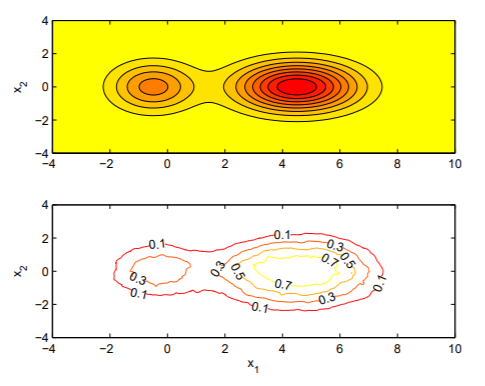
\includegraphics{images/density_levels.png}
    \caption[Density levels]{Density levels in two 2D data clusters and the corresponding rank levels \cite{qian2013spectral}.}
    \label{fig:density_levels}
\end{figure}

\begin{figure}[!ht]
    \centering
    \subfloat[Cut value in terms of $k$]
    {{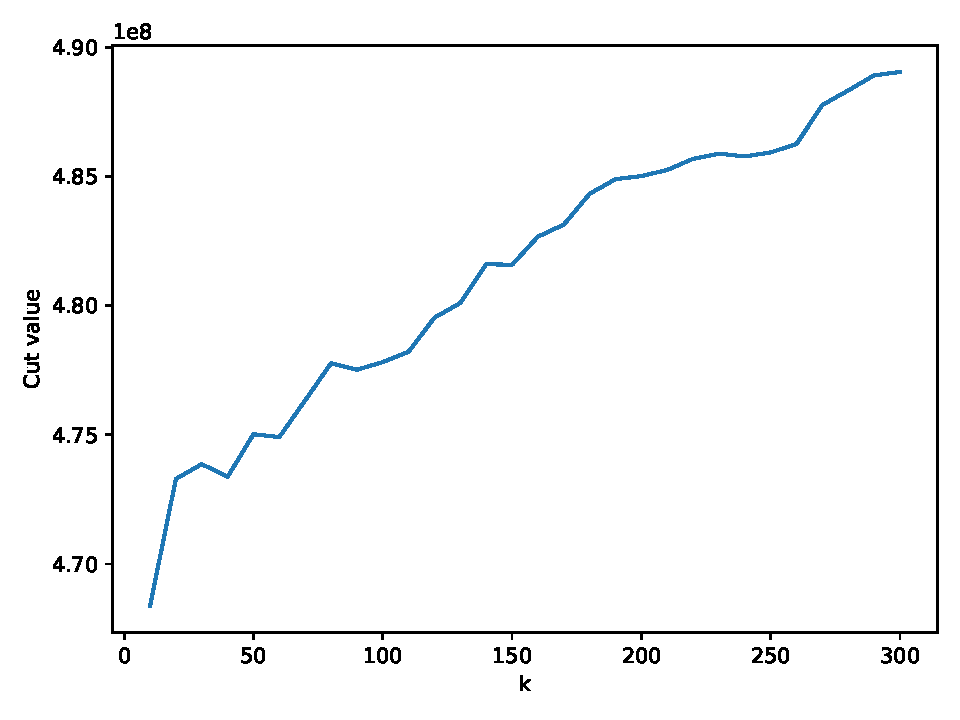
\includegraphics[width=7cm]{images/test_bad_cuts.pdf} }}%
    \qquad
    \subfloat[Precision in terms of $k$]
    {{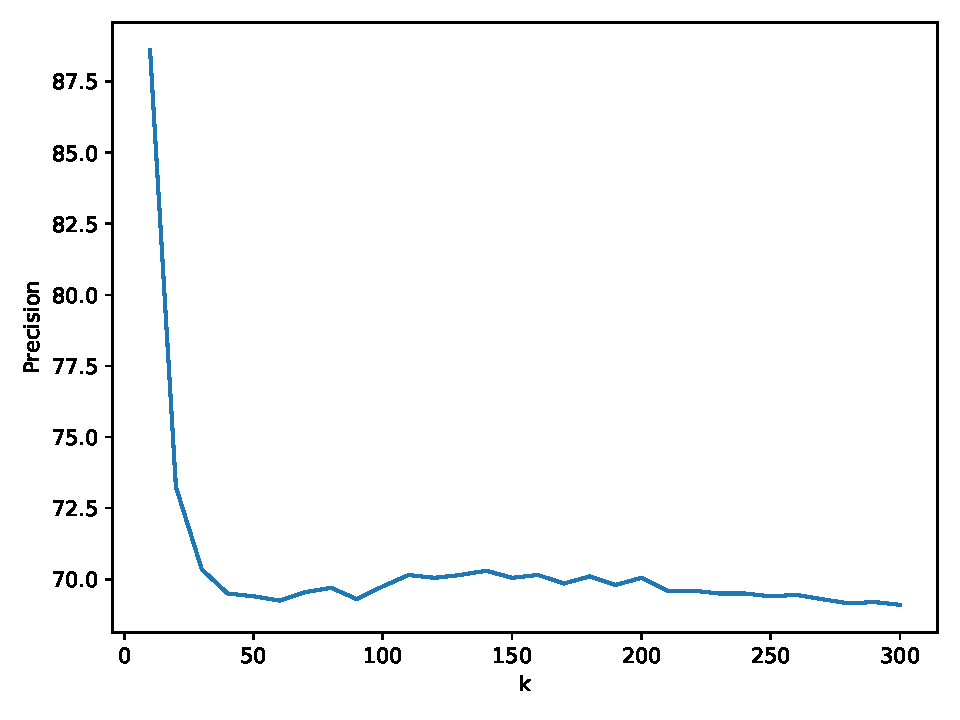
\includegraphics[width=7cm]{images/test_bad_acc.pdf} }}%
    \caption[Iterative scaling]{The importance of $k$ in a case of imbalanced discovery matrix of barcodes $5,6,7,8$.}    \label{fig:cut_acc+_plot}%
\end{figure}

The results by Qian et al. show indicate that RMD is superior to other algorithms if the data is imbalanced. Moreover, their article shows that RMD performs comparably well when the data is balanced.

